\documentclass[a4paper,num-refs]{oup-contemporary}
% \RequirePackage[2020-02-02]{latexrelease}
% \documentclass[times, twoside]{zHenriquesLab-StyleBioRxiv}

\journal{gigascience}

\usepackage{graphicx}
\usepackage{siunitx}

%\usepackage{blindtext}
\usepackage{algorithm}
\usepackage{algpseudocode}

\title{MaBoSS for HPC environments: Implementations of the continuous time Boolean model simulator for large CPU clusters and GPU accelerators}
% \shorttitle{MaBoSS for HPC environments}

% Use letters for affiliations, numbers to show equal authorship (if applicable) and to indicate the corresponding author
\author[1,\authfn{1}]{Adam Šmelko}
\author[2]{Miroslav Kratochvíl}
\author[3,4,5]{Emmanuel Barillot}
\author[3,4,5]{Laurence Calzone}
\author[3,4,5,\authfn{1}]{Vincent Noël}

\affil[1]{Department of Distributed and Dependable Systems, Charles University, Prague, Czech Republic}
\affil[2]{Luxembourg Centre for Systems Biomedicine, University of Luxembourg, Esch-sur-Alzette, Luxembourg}
\affil[3]{Institut Curie, Université PSL, F-75005, Paris, France}
\affil[4]{INSERM, U900, F-75005, Paris, France}
\affil[5]{Mines ParisTech, Université PSL, F-75005, Paris, France}

\authnote{\authfn{1}smelko@d3s.mff.cuni.cz; vincent.noel@curie.fr}

\papercat{Paper}

\runningauthor{Šmelko et al.} 

\jvolume{00}
\jnumber{0}
\jyear{2023}

\begin{document}

\begin{frontmatter}
\maketitle

%TC:break Abstract
%the command above serves to have a word count for the abstract
\begin{abstract}
Computational models in systems biology are becoming more important with the advancement of experimental techniques to query the mechanistic details responsible for leading to phenotypes of interest. In particular, Boolean models are well fit to describe the complexity of signaling networks while being simple enough to scale to a very large number of components. With the advance of Boolean model inference techniques, the field is transforming from an artisanal way of building models of moderate size to a more automatized one, leading to very large models. In this context, adapting the simulation software for such increases in complexity is crucial. 
We present two new developments in the continuous time Boolean simulators: MaBoSS.MPI, a parallel implementation of MaBoSS which can exploit the computational power of very large CPU clusters, and MaBoSS.GPU, which can use GPU accelerators to perform these simulations. 
\end {abstract}
%TC:break main
%the command above serves to have a word count for the abstract

\begin{keywords}
Computational Biology | High Performance Computing | Boolean models
\end{keywords}
\end{frontmatter}

\section{Introduction}

Biological systems are large and complex, and understanding their internal behavior remains critical for designing new therapies for complex diseases such as cancer.
A crucial approach in this endeavor is building computational models from existing knowledge and analyzing them to find intervention points and to predict the efficacy of new treatments.
Many different frameworks have been used to describe biological systems, from quantitative systems of differential equations to more qualitative approaches such as Boolean models.
While the former seems more adapted to represent complex behavior, such as non-linear dependencies, the latter is being increasingly used because of its capability to analyze very large systems.
Many Boolean models have been built to describe biological systems to tackle a variety of problems: from understanding fundamental properties of cell cycle~\cite{faure2006cellcycle,sizek2019boolean} to advanced properties of cancer~\cite{fumia_carcinogenesis_2013,montagud2022prostate}.

Historically, the task of building Boolean models involved reading an extensive amount of literature and summarizing it in a list of essential components and their interactions.
More recently, thanks to advances in databases listing such interactions~\cite{licata2020signor,turei2016omnipath} and to experimental techniques providing information on a bigger number of components, the automatic methods have been designed to infer Boolean formulas from the constraints encoded in the knowledge and the experimental data~\cite{10.1093/bioinformatics/btaa484,chevalier2020synthesis,benevs2023boolean}, allowing construction of large Boolean models.
While this effort faces many challenges, we believe it is a promising way to study the large-scale complexity of biological systems.
However, in order to analyze the dynamic properties of such large Boolean models, we need to develop efficiently scalable simulation tools.

Here, we present adaptations of MaBoSS~\cite{stoll2012continuous, stoll2017maboss} --- a stochastic Boolean simulator that performs estimations of state probability trajectories based on Markov chains -- to modern HPC computing architectures, which provide significant speedups of the computation, thus allowing scrutinization and analysis of much larger boolean models.
The main contributions comprise of two new implementations of MaBoSS:
\begin{itemize}
    \item MaBoSS.GPU, a GPU-accelerated implementation of MaBoSS, which is designed to exploit the computational power of massively parallel GPU hardware.
    \item MaBoSS.MPI, a parallel implementation of MaBoSS which can scale to multinode environments, such as large CPU clusters.
\end{itemize}

The source code of the proposed implementations is publicly available at their respective GitHub repositories\footnote{\url{https://github.com/sysbio-curie/MaBoSS.GPU}} \footnote{\url{https://github.com/sysbio-curie/MaBoSS-env-2.0}}. We also provide the scripts, presented plots, data and instructions to reproduce the benchmarks in the replication package\footnote{\url{https://github.com/asmelko/gigascience24-artifact}}.

To showcase the utility of the new implementations, we performed benchmarking on both existing models and large-scale synthetic models. As the main results, MaBoSS.GPU may provided over 200\texttimes\ speedup over the current version of MaBoSS on a wide range of models using contemporary GPU accelerators, and MaBoSS.MPI is capable of almost linear performance scaling with added HPC resources, allowing similar speed-ups by utilizing the current HPC infrastructures.

\section{Background}

\subsection{Boolean signaling models}

% this is very cool but can we simply refer to the maboss paper? or no one took care to formalize this properly yet?

A Boolean signaling model consists of $n$ nodes which are either active or inactive, gaining values 1 or 0 respectively. The \emph{state} of the whole model is represented by a vector $S$ of $n$ Boolean values where $S_i$ represents the value of the $i$-th node. We denote the set of all possible states as $\mathcal{S} = \{0, 1\}^n$; thus $|\mathcal{S}| = 2^n$. 

Interactions in the model are described as transitions between two states. A single state can have multiple transitions to other states with assigned transition probabilities. In turn, a Boolean network is represented as a directed weighted graph $G = (\mathcal{S}, \rho)$, where $\rho: \mathcal{S} \times \mathcal{S} \rightarrow [0, \infty)$ is a transition function generating \emph{transition rates}. For convenience, it holds that:
\[ \rho(S, S') = 0 \iff \text{there is no transition from}\ S\ \text{to}\ S' \]
MaBoSS simulates the \emph{asynchronous update strategy}, where at most a single node changes its value in each transition --- consequently, a state $S$ can have at most $n$ possible transitions.

To determine the possible transitions, each node follows the \emph{Boolean logic} $\mathcal{B}_i: \mathcal{S} \rightarrow [0, \infty)$, which determines the expected Poisson-process rate of transitioning to the other value. If $\mathcal{B}_i(S) = 0$, then the transitions at node $i$ is not allowed in state $S$.
Given this formalization, the simulation can be also viewed as a continuous-time Markov process.

MaBoSS algorithm simulates the above process to produce stochastic \emph{trajectories}: sequences of states $S^0, S^1, \dots, S^k$ and time points $t^0 < t^1 < \dots < t^k$ where $t^0 = 0$ and $S^0$ is the initial state, and for each $i \in \{0, \dots, k-1\}$, $S^i$ transitions to $S^{i+1}$ at time $t^{i+1}$. The simulation ends either by a timeout when reaching the maximal allowed time, or by reaching a fixed point state with no outgoing transitions. The algorithm for a single iteration of the trajectory simulation is given explicitly in Algorithm~\ref{alg:iter}.

\begin{algorithm}
\caption{A single iteration of the MaBoSS simulation of a trajectory, given the state $S$ and time $t$.}
\label{alg:iter}
\begin{algorithmic}[1]
\Procedure{TrajectorySimulationStep}{S, t}
\State $\rho_1 \gets \mathcal{B}_1(S), \dots, \rho_n \gets \mathcal{B}_n(S)$ \Comment compute transition rates
\State $r \gets \text{random}([0, \sum_{i=1}^n \rho_i))$
\State $i \gets \min_i \sum_{j=1}^{i-1} \rho_j \leq r < \sum_{j=1}^{i} \rho_j$ \Comment select a node for flipping
\State $S'\gets S\ \text{with the $i$-th bit flipped}$
\State $u \gets \text{random}([0, 1])$
\State $\delta t \gets -\frac{\ln u}{\sum_{i=1}^n \rho_i}$
\State \textbf{return} $(S', t + \delta t)$
\EndProcedure
\end{algorithmic}
%TODO this should be in a float/figure (\begin{algorithm} etc)
\end{algorithm}

To obtain a good overview of the Markovian process, multiple trajectories are generated and aggregated in a compound trajectory statistics. Commonly obtained statistics include:
\begin{itemize}
    \item \emph{Network state probabilities on a time window} --- Trajectory states are divided by their transition times into time windows based on the time intervals specified by a window size. For each window, the probability of each state is computed as the duration spent in the state divided by the window size. The probabilities of the corresponding windows are then averaged across all subtrajectories.
    \item \emph{Final states} --- The last sampled states from the trajectories are used to compute a final state distribution.
    \item \emph{Fixed states} --- All reached fixed points are used to compute a fixed state distribution.
\end{itemize}

To maintain the brevity in the statistics, MaBoSS additionally allows marking some nodes \emph{internal}.
This is useful because nodes that are not ``interesting'' from the point of final result view occur quite frequently in Boolean models, and removing them from statistics computation often saves a significant amount of resources.

\subsection{Computational complexity of MaBoSS algorithm in parallel}

\subsubsection{Simulation complexity}

% TODO this paragraph needs friggin references to the algorithm figure -- took me a while to see where to get the "all other parts"
We estimate the time required to simulate $c$ trajectories as follows:
For simplification, we assume that a typical Boolean logic formula in a model of $n$ nodes can be evaluated in $\mathcal{O}(n)$ (this is a very optimistic but empirically valid estimate). With that, the computation of all possible transition rates can be finished in $\mathcal{O}(n^2)$. The selection of the flipping bit can be finished in $\mathcal{O}(n)$, and all other parts of the iteration can finish in $\mathcal{O}(1)$. In total, the time complexity of one iteration is $\mathcal{O}(n^2)$. If we simulate $c$ trajectories with an upper bound of trajectory length $u$, the simulation time is in $\mathcal{O}(c \cdot u \cdot n^2)$.

In an idealized PRAM model with infinite parallelism, we can optimize the algorithm in the following ways:
\begin{itemize}
    \item Given $c$ processors, all trajectory simulations can be performed in parallel, reducing the time complexity to $\mathcal{O}(m \cdot n^2)$.
    %TODO might be useful to explicitly note that this doesn't include result aggregation (and link to the section)
    \item With $n$ processors, the computation of transition rates in the simulation can be done $\mathcal{O}(n)$ time, and the selection of the flipping bit can be done in $\mathcal{O}(\log{n})$ time using a parallel prefix sum, giving $\mathcal{O}(n)$ time for a single iteration.
\end{itemize}
Thus, using a perfect parallel machine with $c \cdot n$ processors, the computation time can be reduced to $\mathcal{O}(u \cdot n)$. Notably, the $\mathcal{O}(u)$ simulation steps that must be performed serially remain a major factor in the whole computation time.

\subsubsection{Statistics aggregation}

The aggregation of the statistics from the simulations is typically done by updating a shared associative structure indexed by model states, differing only in update frequency between the three kinds of collected statistics.

If the associative structure is implemented as a hashmap, the updates can be done in $\mathcal{O}(1)$ for a single process. With multiple processors, the algorithm may hold partial versions of the hashmap for each processor, and aggregate all of them at the end of computation, which can be done in $\mathcal{O}(\log{c} \cdot m)$ using $c$ processors, assuming the maximal size of statistic to be $m$.

As an interesting detail, the hash structures pose a surprising constant-factor overhead. In networks where most nodes are internal, the hash map may be replaced by a fixed-size multidimensional array that holds an element for all possible combinations of external node values (basically forming a multidimensional histogram). We discuss the impact of this optimization in the next section.

\section{Implementation}\label{sec:implementation}

\subsection{MaBoSS.GPU}

\subsubsection{Simulation}

In the CPU version of MaBoSS, the simulation part is the most computationally demanding part, with up to 80\% of MaBoSS runtime spent by just evaluating the Boolean formulas (the exact number depends on the model). The original formula evaluation algorithm in MaBoSS used a recursive traversal of the expression tree, which (apart from other issue) causes memory usage patterns unsuitable for GPUs: the memory required per each core is not achievable in current GPUs, and there are typically too many cache misses~\cite{karlsson2000prefetching}

There are multiple ways to optimize the expression trees for GPUs: One may use a linked data structure that is more cache-friendly such as the van Emde Boas tree layout~\cite{van1975preserving}, or perhaps represent the Boolean formulas as a compact continuous array, or convert it to CNF or DNF bitmasks that can be easily evaluated by vector instructions. We decided to leave the exact representation choice on the compiler, by encoding the expressions as direct code and using the runtime compilation of GPU code~\cite{nvrtc}. Using this technique, the Boolean formulas are compiled as functions into a native binary code, which is directly executed by the GPU. As the main advantage, the formulae are encoded in the instructions, preventing unnecessary fetches of the encoded formulas from other memory. At the same time, the compiler may apply a vast spectrum of optimizations on the Boolean formulas, including case analysis and shortcutting, again resulting in faster evaluation.

A possible drawback of the runtime compilation stems from the relative slowness of the compiler --- for small models, the total execution time of MaBoSS.GPU may be easily dominated by the compilation.

Also, due to the involved implementation complexity, we avoided optimization of the computation of individual trajectories by splitting the Boolean function evaluation to multiple threads (thus missing the factor of $n$ threads from the asymptotic analysis). While such optimization might alleviate some cache pressure and thus provide significant performance improvements, we leave its exploration to future work.

\subsubsection{Statistics aggregation}

For optimizing the statistics aggregation, MaBoSS.GPU heavily relies on the fact that the typical number of non-internal nodes in a real-world MaBoSS model rarely exceeds 10 nodes, regardless of the size of the model. This relatively low number of states generated by non-internal nodes allows us to materialize the whole statistics structure (called ``histogram'') as a fixed-size array (rarely exceeding $2^10$ elements).

This approach allows us to avoid storing the states as the keys, and gives a simple approach that can map the state to the histogram index using simple bit masking and shifting instructions. Further, we use sevelra well-known GPU histogram update optimizations to improve the performance, including as shared memory privatization and atomic operations.

\subsection{MaBoSS.MPI}

MaBoSS.MPI is a straightforward extension of the original MaBoSS CPU code to the MPI programming interface.
Briefly, each thread is assigned to compute a single trajectory at once, progressively collecting the results into a privatized hashmap-based statistics aggregation structure. The total amount of trajectory tasks is evenly split among the MPI nodes, adding a second layer of parallelism.

Once all trajectory simulations are finished and the statistics are computed for each thread, the intermediate data are reduced into the final result using MPI collective operations.


% MaBoSS' CPU implementation already offered parallelism, allowing to use multiple CPU cores to compute the multiple trajectories. However, this implementation stays limited to a single machine CPU, and its scalability suffers from a very intensive memory usage. Furthermore, with the increasing number of nodes in Boolean models, the need for very large number of trajectories leads to large simulation time. 
% To tackle this, we decided to extend this implementation and add another layer of parallelism using MPI. In this implementation, the simulation of the trajectories is not only distributed on multiple cores, but on the multiple cores of multiple MPI nodes. By using this implementation, we are able to exploit the large CPU clusters available in HPC centers. 
% The implementation of this MPI implementation is straightforward, and consists in distributing the invidivual trajectories even further, first on MPI nodes and then on the CPU cores of the MPI node. Once the trajectories are simulated, the statistics are first computed for each MPI nodes, and then the global results is computer from the results of each MPI nodes. 


\section{Results}

To evaluate the impact of the implemented optimizations, we present the results of performance benchmarks for MaBoSS.GPU and MaBoSS.MPI by comparing their runtimes against the original CPU implementation. To obtain a comprehensive overview of achievable results, we used both real-world models and synthetic models with varying sizes.

\subsection{Benchmarking Methodology}

% TODO: ok well, here you have a grande totale insane of 3 models, and decide to omit the size of the middle one by saying "yeah between 10 and 133" :D
For the benchmarks, we used $3$ real-world models of $10$, $XXX$ and $133$ nodes (\texttt{cellcycle}~\cite{faure2006cellcycle}, \texttt{sizek}~\cite{sizek2019boolean} and \texttt{Montagud}~\cite{montagud2022prostate}). In order to test the scalability of the GPU and MPI implementation, we also created several synthetic models with up to $1000$ nodes. Synthetic models were designed in a way such that the length of each trajectory is predictable, and the models have no stable states. Also, the number of non-internal nodes was kept low (10 nodes) to enable the usage of the histogram optimization.
%TODO here it would be nice to calm down stupid questions like "ok how realistic are the models actually" by pointing out that they are in the repository or something.

The GPU implementation benchmarks were run on a datacenter-grade NVIDIA Tesla A100 GPU and a consumer-grade NVIDIA RTX 3070 Laptop GPU. The CPU implementation benchmarks were run on a 32-core Intel Xeon Gold 6130 CPU with multithreading. The CPU implementation was compiled with GCC 13.2.0, and the GPU implementation was compiled with CUDA 12.2. Each measurement was repeated $10$ times, and the average runtime was used as the final results after removing the outliers.
%TODO: stats trigger: how did you remove the outliers? Manual QA? What caused the outliers?

The MPI implementation benchmarks were run on the MareNostrum 4 supercomputer.
% TODO link to MN spec (I think they have a paper)

\subsection{Performance of MaBoSS.GPU}

\begin{figure}
    \centering
    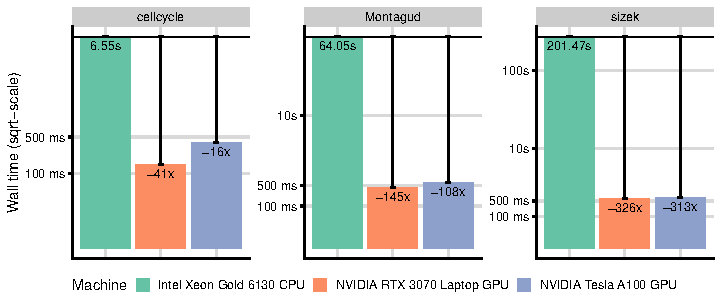
\includegraphics[width=\linewidth]{Figures/real.pdf}
    \caption{Wall time comparison of MaBoSS and MaBoSS.GPU on real-world models. Each model is simulated with 1 million trajectories.}
    % TODO it's slightly inconvenient that the plot legend only describes hardware; in turn the whole thing looks like you're benchmarking the hardware instead of the actual sofware implementations. Suggest using: MaBoSS (CPU), MaBoSS.GPU (RTX3070), MaBoSS.GPU (A100).
    \label{fig:real}
\end{figure}

% TODO above you're putting the Montagud/Sizek/whatever names into \texttt. I'd recommend using \textsc and doing it veeery consistently everywhere. Just for the general purpose of sparking the benchmark-nerd imaginations.
In Figure~\ref{fig:real}, we compare the wall time of the CPU and GPU implementations on real-world datasets. The GPU implementation is faster than the CPU implementation on all models, and the speedup shows to be more significant on the models with more nodes and longer trajectories. On the Montagud model with 133 nodes, but a relatively short average trajectory, we achieve $145\times$ speedup. On a slightly smaller Sizek model with a longer average trajectory, the speedup is up to $326\times$. 

\begin{figure}
    \centering
    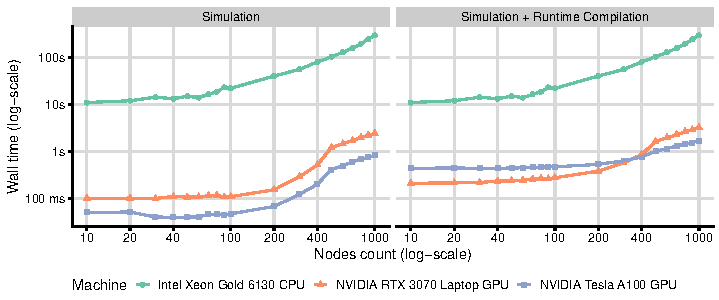
\includegraphics[width=\linewidth]{Figures/nodes.pdf}
    \caption{Wall time comparison of MaBoSS and MaBoSS.GPU on synthetic models. Each model is simulated with 1 million trajectories. The two panels differ by inclusion of the runtime GPU code compilation, showing its impact on total run time.}
    \label{fig:synth}
\end{figure}

Figure~\ref{fig:synth} shows much finer performance progression on synthetic models. We observed that the CPU variant starts to progress steeper at around the $100$ nodes boundary. We assume that the implementation hits the cache size limit, and the overhead of fetching the required data from the memory becomes dominant. The same can be observed in the GPU variant later at around $200$ nodes. Expectably, the cache-spilling performance penalty is much more significant on GPUs. Overall, the results suggest that the optimization of dividing transition rate computations among multiple threads, as mentioned in the previous section XXX TODO REF XXX, may provide a better speedup for bigger models, as it alleviates the register and cache pressure.
% TODO danger there's a non-commented TODO above. Add an actual \ref if possible.

\begin{figure}
    \centering
    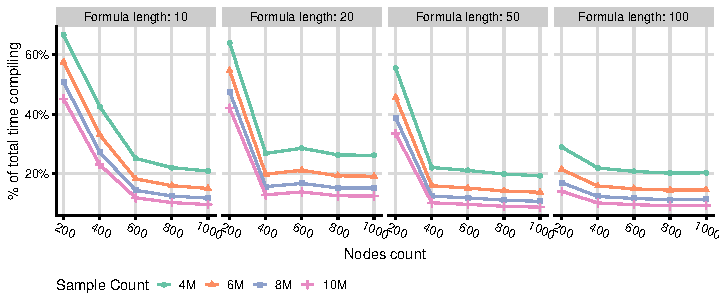
\includegraphics[width=\linewidth]{Figures/nodes-compilation-big-NVIDIA Tesla A100 GPU.pdf}
    \caption{The time spent in the runtime compilation of the Boolean formulas simulating models with varying numbers of nodes, trajectories, and formula lengths.}
    % TODO: what happens if we swap the sample count (color) with formula length (facet) ?
    % Also, it might be much better to have the percentages as logarithmic scale. (most of the space is now killed by the single 200node 10formula point)
    % TODO: "sample count" in the legend is not defined anywhere around, maybe say "total trajectories" ?
    \label{fig:comp}
\end{figure}

Additionally, Figure~\ref{fig:synt} shows the total runtime of the GPU implementation including the runtime compilation step. Comparing the panels, we observe that that the relative runtime compilation overhead quickly disappears with increasing model size. Figure~\ref{fig:comp} shows the results of a more detailed benchmarks for this scenario, as run on the NVIDIA Tesla A100 GPU. We observed that the compilation time is linearly dependent on the number of nodes and formula lengths (measured in the number of occurring nodes). Notably, as soon as the simulation becomes more complex (e.g., by increasing the number of nodes or simulated trajectories), the compilation time becomes relatively negligible even for models with unrealistically long formulae. This suggests that the runtime compilation is a viable optimization methodology also for much larger models.

\subsection{Performance of MaBoSS.MPI}

%TODO achtung, the figure DPI is somehow messed up and the letters are too tiny.
%TODO: might be better to merge the figures into one (2 facets)
%TODO: it's nice that there's a trend on the diagonal but that kinda looks like we're hiding fluctuations or small off-angle, can we scale the thing into a visibly horizontal straight line?
%  - multiply the walltime by the number of cores to produce the realistic totalwastedtime
%  - divide the speedup by the number of cores invested (to show speedup per investment)

\begin{figure}%[tbhp]
\centering
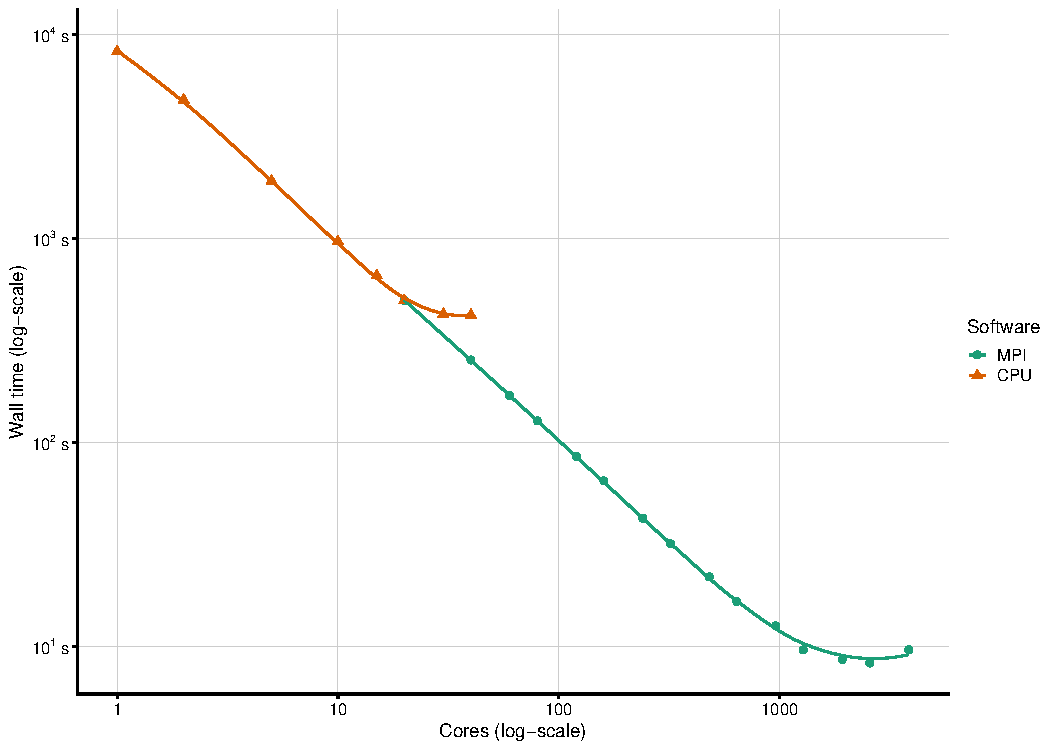
\includegraphics[width=.8\linewidth]{Figures/sizek_mpi.pdf}
\caption{Scalability results of MPI implementation on Sizek model with 20 cores per MPI node.}
\label{fig:sizek_results}
\end{figure}

Figure~\ref{fig:sizek_results} shows the efficiency of the MaBoSS.MPI implementation on the Sizek model. We ran multiple suites, ranging from a single MPI node up to 192 nodes, each running 20 cores. We can observe a close-to-linear speedup of up to 64 MPI nodes (1280 cores), and a plateau for larger suites (Figure~\ref{fig:sizek_results}, green). This can be explained by hitting an expectable bottleneck in parallelization overhead and MPI communication cost when the problem is divided into too many small parts.

\begin{figure}%[tbhp]
\centering
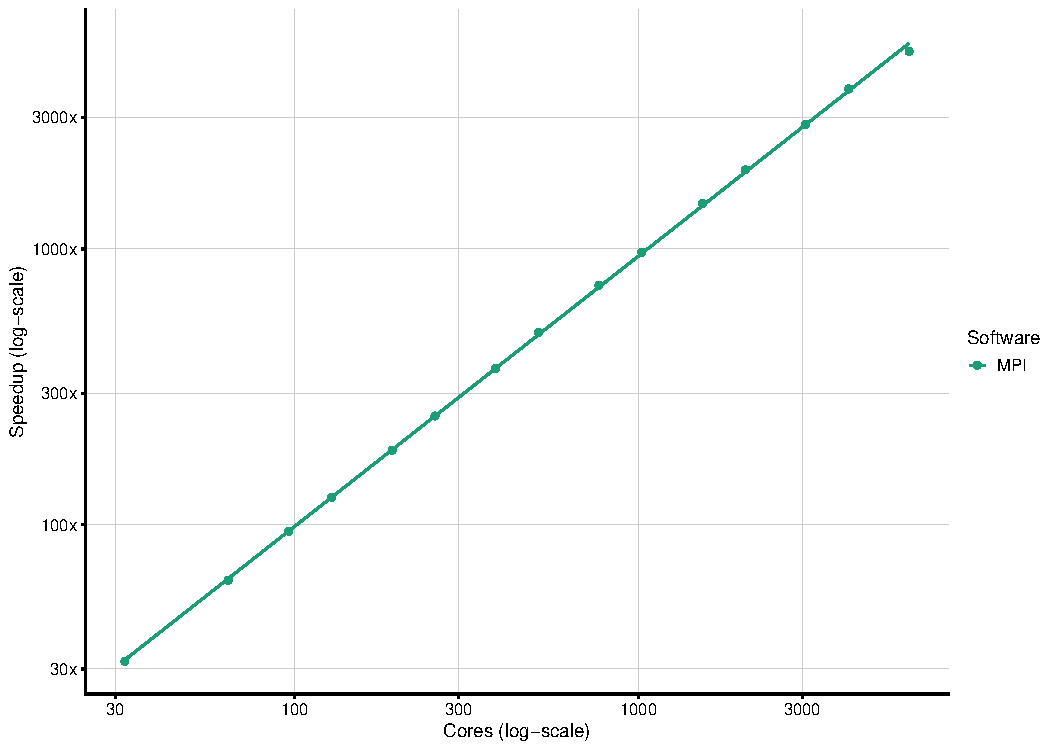
\includegraphics[width=.8\linewidth]{Figures/synth_mpi_speedup.pdf}
\caption{Speedup scaling of MPI implementation on a synthetic model with 1000 nodes and 32 cores per MPI node.}
\label{fig:synthetic_results}
\end{figure}

To stress the scalability of the implementation, we also used a synthetic model with 1000 nodes. We simulated this model on 32 cores per MPI node, on 1 to 192 nodes (32 to 6144 cores). The obtained speedups are summarized in Figure~\ref{fig:synthetic_results}. Using this configuration, the simulation time decreases from 20 hours on 1 MPI node to 430 seconds on 192 nodes. As expected, the plateau in the speedup was not observed in simulations that involve larger models.

% We simulated a cell cycle model by Sizek et al.\cite{sizek2019boolean} (Figure~\ref{fig:sizek_results}). A comparison of execution times of MaBoSS v2.5.3 and v2.4.0 using 40 cores and one million individual simulations showed a considerable (3×) speed-up between the pre- and post-optimisation versions, which is mostly due to optimised memory usage (figure 2, purple vs red). We used the same test with the MPI implementation of MaBoSS, using 20 cores for each MPI node, from 1 MPI node up to 192 MPI nodes. We can observe a very good speedup (>50x) up to 64 MPI nodes (1.28k cores), and a plateau for larger setups (Figure 7, green). This is probably due the very short simulation time (10s) for that setup and the minimum overhead for such a parallel simulation, and needs testing on larger simulations.


% In order to explore larger model sizes, we created a synthetic model with 1000 nodes (Figure~\ref{fig:synthetic_results}). We simulated this model on 32 cores per MPI node, on 1 to 192 MPI nodes (32 to 6144 cores). With this dataset, the simulation time goes from 20 hours on 1 MPI node to 430 seconds on 192 nodes. As we hypothesised, with larger simulation times, a decline in the speedup was not observed as in the previous example 
% The MaBoSS benchmarking measurements described in this section were performed on MareNostrum 4.

% \begin{figure}%[tbhp]
% \centering
% 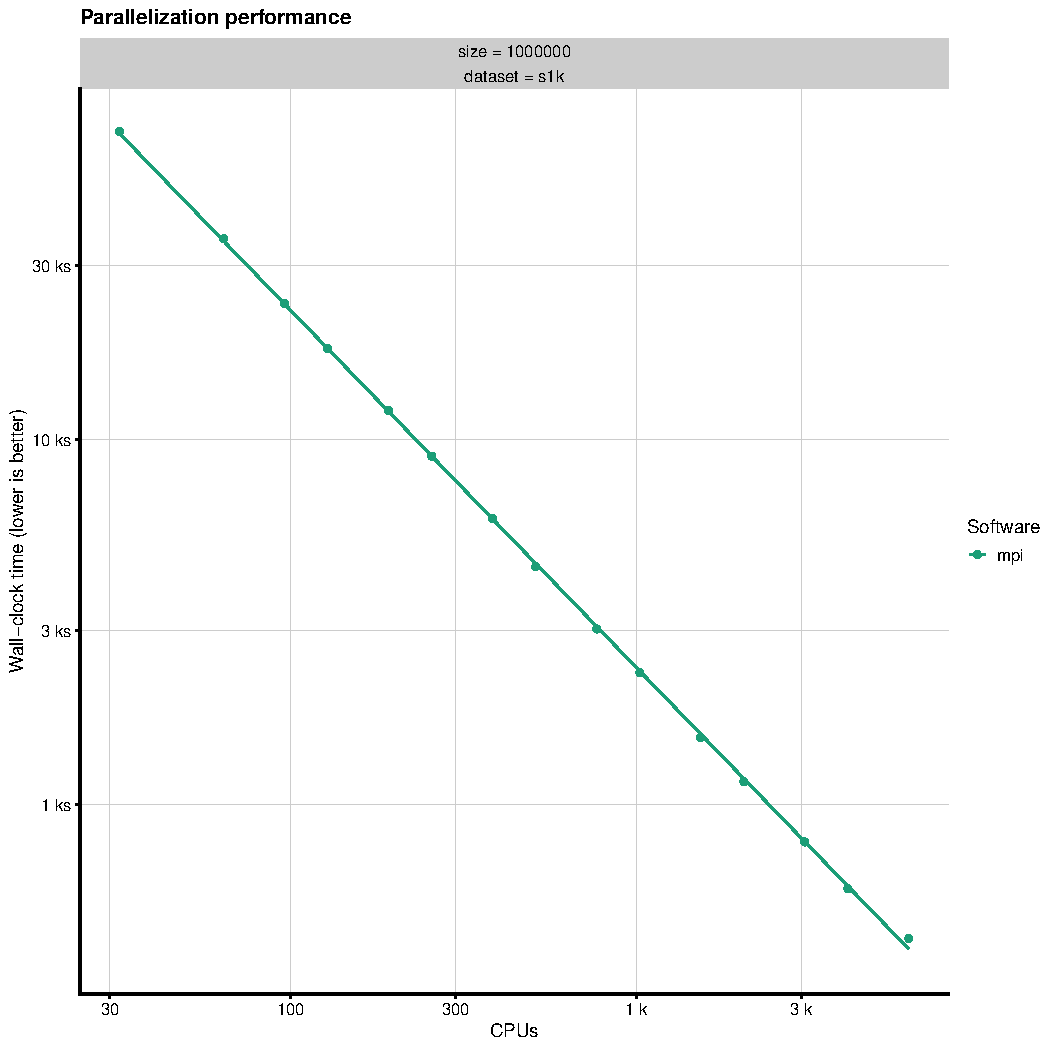
\includegraphics[width=.8\linewidth]{Figures/large_model.pdf}
% \caption{Scalability results for synthetic model with 1000 nodes}
% \label{fig:synthetic_results}
% \end{figure}

%\begin{figure}%[tbhp]
%\centering
%\includegraphics[width=.8\linewidth]{Figures/Figure_1}
%\caption{Placeholder image of Iris with a long example caption to show justification setting.}
%\label{fig:computerNo}
%\end{figure}

\section{Conclusions}

In this work, we presented two new implementations of MaBoSS tool, a continuous time Boolean model simulator, both of which are designed to enable utilization of the HPC computing resources: MaBoSS.GPU is designed to exploit the computational power of massively parallel GPU hardware, and MaBoSS.MPI enables MaBoSS to scale to many nodes of HPC clusters via the MPI framework. We evaluated the performance of these implementations on real-world and synthetic models and demonstrated that both variants are capable of providing significant speedups over the original CPU code. The GPU implementation shows 145--326\texttimes\ speedup on real-world models, and the MPI implementation delivers a close-to-linear strong scaling on big models.

Overall, we believe that the new MaBoSS implementations enable simulation and exploration of the behavior of very large, automatically generated models, thus becoming a valuable analysis tool for the systems biology community.

\subsection{Future work} 

During the development, we identified several optimization directions that could be taken by researchers to further scale up the MaBoSS simulation approach.

Mainly, the parallelization scheme used in MaBoSS.GPU could be enhanced to also parallelize over the evaluation of Boolean formulas. To avoid GPU thread divergence, this would however require a specialized Boolean formula representation, entirely different from the current version of MaBoSS; likely even denying the relative efficiency of the use of runtime compilation. On the other hand, this optimization might decrease the register pressure created by holding the state data, and thus increase the performance on models with thousands of nodes.

In the long term, easier optimization paths might lead to sufficiently good results: For example, backporting the GPU implementation improvements back to the MaBoSS CPU implementation could improve the performance even on systems where GPU accelerators are not available. Similarly, both MaBoSS.GPU and MaBoSS.MPI could be combined into a single software that executes distributed GPU-based analysis over multiple MPI nodes, giving a single high-performance solution for extremely large problems.

\section{Acknowledgements}
We thank Gautier Stoll for his guidance and fruitful discussion.

\section{Funding}
%TODO the permed ack wasn't right, it should be:
he research leading to these results has received funding from the European Union's Horizon 2020 Programme under the PerMedCoE Project (\url{http://www.permedcoe.eu}), grant agreement n\textsuperscript{o}~951773.
% This work was supported by the European Commission under the PerMedCoE project [H2020-ICT-951773]
The project was partially supported by Charles University, SVV project number~260698.


% \section*{Bibliography}
\bibliography{bibliography}

%% You can use these special %TC: tags to ignore certain parts of the text.
%TC:ignore
%the command above ignores this section for word count
% \onecolumn
% \newpage

%%%%%%%%%%%%%%%%%%%%%%%%%%%%%
% Supplementary Information %
%%%%%%%%%%%%%%%%%%%%%%%%%%%%%
%\captionsetup*{format=largeformat}
%\section{Something about something} \label{note:Note1} 
%Something

%TC:endignore
%the command above ignores this section for word count

\end{document}
